\documentclass[10pt,a4j,dvipdfmx]{jarticle}
%---------------------------------------------------
\usepackage{hyperref}
\usepackage{pxjahyper}
\usepackage{bm}
\usepackage{graphicx}
\usepackage{amssymb,amsmath}
\usepackage{ascmac}
\usepackage{float}
\usepackage{setspace}
\usepackage[dvips,usenames]{color}
\usepackage{colortbl}
\usepackage{algorithm}
\usepackage{algorithmic}
\usepackage{setspace}
\usepackage{subfigure}
\usepackage{here}
\usepackage[deluxe,bold]{otf}
\usepackage[haranoaji]{pxchfon}
\usepackage{redeffont}
\usepackage{listings,jvlisting} %日本語のコメントアウトをする場合jvlisting(もしくはjlisting)が必要
\usepackage{booktabs}
\usepackage{siunitx}
\usepackage{fancybox}
\usepackage{tikz}
%---------------------------------------------------
% \definecolor{bl}{rgb}{0.94,0.97,1}
% \definecolor{gr}{rgb}{0.5,0.5,0.5}
% \makeatletter
% \def\section{\newpage\@startsection {section}{1}{\z@}{2.3ex plus -1ex minus -.2ex}{2.3 ex plus .2ex}{\Large\bf}}
% \makeatother
%---------------------------------------------------
\setlength{\textwidth}{160truemm}
\setlength{\textheight}{240truemm}
\setlength{\topmargin}{-14.5truemm}
\setlength{\oddsidemargin}{-0.5truemm}
\setlength{\headheight}{0truemm}
\setlength{\parindent}{1zw}
\setlength{\abovedisplayskip}{-2pt} % 数式上部のマージン
\setlength{\belowdisplayskip}{-2pt} % 数式下部のマージン
%---------------------------------------------------
\setstretch{1.2}
%---------------------------------------------------
\renewcommand{\subfigtopskip}{5pt}	% 図の上の隙間。上図の副題と下図の間。
\renewcommand{\subfigbottomskip}{0pt} % 図の下の隙間。副題と本題の間。
\renewcommand{\subfigcapskip}{-6pt}	% 図と副題の間
\renewcommand{\subcapsize}{\scriptsize} % 副題の文字の大きさ
\newcommand{\mysection}[1]{\vspace{-20pt}\section{#1}}
\newcommand{\mysubsection}[1]{\vspace{-20pt}\subsection{#1}}
\newcommand{\mysubsubsection}[1]{\vspace{-10pt}\subsubsection{#1}}
\renewcommand{\lstlistingname}{ソースコード}
\newcommand{\tsuyo}[1]{\textbf{\textgt{#1}}}
%---------------------------------------------------
% ヘッダーとフッターの設定
\usepackage{fancyhdr}
\rhead{ME2208\CID{8705}橋尚太郎}
\chead{}
\lhead{情報数理工学 課題1 1章の問題}
\cfoot{\thepage}

\rfoot{}
\begin{document}
%---------------------------------------------------
\setlength{\abovedisplayskip}{1.5pt} 
\setlength{\belowdisplayskip}{0pt}
%---------------------------------------------------
%ここからソースコードの表示に関する設定
\lstset{
  basicstyle={\ttfamily},
  identifierstyle={\small},
  commentstyle={\smallitshape},
  keywordstyle={\small\bfseries},
  ndkeywordstyle={\small},
  stringstyle={\small\ttfamily},
  frame={tb},
  breaklines=true,
  columns=[l]{fullflexible},
  numbers=left,
  xrightmargin=0zw,
  xleftmargin=3zw,
  numberstyle={\scriptsize},
  stepnumber=1,
  numbersep=1zw,
  lineskip=-0.5ex
}
%ここまでソースコードの表示に関する設定
%---------------------------------------------------

\thispagestyle{empty}
\begin{spacing}{1}

\begin{center}
{\Large 明石工業高等専門学校専攻科 \\[1truecm]
情報数理工学 課題1} \\[3.5truecm]
\huge \tsuyo{1章の問題} \\
% \LARGE Digital Ociloscope and Waveform Processing\\
[4truecm]
\Large ME2208 \CID{8705}橋 尚太郎 \\
(機械・電子システム工学専攻2年) \\[1truecm]
提出年月日:\today
\end{center}

% \begin{center}
% \vspace*{3.5cm}
% {\Huge トランジスタ回路の設計}\\
% \vspace*{12.5cm}
% {\Large 電気情報工学科4年後期}\\
% {\Large 電気電子工学実験II}\\
% \vspace*{1cm}
% \end{center}

\end{spacing}
\clearpage
\pagenumbering{arabic}
\pagestyle{fancy}
\setlength{\headheight}{5truemm}

\mysection{Prblem Set 1.2}

\begin{description}
  \setlength{\parskip}{0cm} % 段落間
  \setlength{\itemsep}{0cm} % 項目間
  \item[8 (a) 回答] Tomは、3 回握手をした。
  \item[8 (b) 回答] Tomの妻は、3 回握手をした。
\end{description}

問題の解を与えるグラフを下図に示す。
Coupleは、夫婦の内、夫、妻のどちらかを表す。
\\


\begin{tikzpicture}[every node/.style={circle,draw}]
  \node (A) at (12.5, 2) {Couple 1};
  \node (B) at (7, 0) {Couple 2};
  \node (C) at (1.5, 2) {Couple 2};
  \node (D) at (0, 7) {Couple 3};
  \node (E) at (2.5, 11) {Couple 3};
  \node (F) at (7, 14) {Tom's Couple};
  \node (G) at (10.5, 11) {Tom's Couple};
  \node (H) at (14, 7) {Couple 1};
  \foreach \u \v in {A/B, A/C, A/D, A/E, A/F, A/G, B/D, B/E, B/F, B/G, D/F, D/G}
      \draw (\u) -- (\v);
\end{tikzpicture}

\mysection{Problem Set 1.8}

\begin{description}
  \setlength{\parskip}{0cm} % 段落間
  \setlength{\itemsep}{0cm} % 項目間
  \item[8 回答] $p=p_1\cdot p_2$, $q=p_1\cdot q_2+p_2 \cdot q_1$
\end{description}
% \section{はじめに}
トランジスタの基本的な増幅回路であるエミッタ接地増幅回路を設計する。
原理の説明と電子回路シミュレーションソフトによる演習を並行して行うことで、電子回路の設計方法を習得する。
シミュレーションソフトは、LTspiceを用いる。

\mysubsection{2SC1815の直流増幅率測定}
\begin{description}
  \setlength{\parskip}{0cm} % 段落間
  \setlength{\itemsep}{0cm} % 項目間
  \item[ゴール] トランジスタの直流電流増幅率を測定する。
  \item[キーワード] 直流増幅率
\end{description}

\begin{description}
  \setlength{\parskip}{0cm} % 段落間
  \setlength{\itemsep}{0cm} % 項目間
  \item[課題1] 専用測定器を用いてトランジスタの直流電流増幅率を測定してください。
\end{description}
% \mysection{トランジスタの基本特性について}
トランジスタは小さな信号を大きな信号に増幅できる特性を持つ半導体素子である。
3つの電極は、E(エミッタ) C(コレクタ) B(ベース) で構成される。今回は、NPNトランジスタを扱う。

\begin{description}
  \setlength{\parskip}{0cm} % 段落間
  \setlength{\itemsep}{0cm} % 項目間
  \item[ゴール] $I_E$-$V_{BE}$ 特性、$I_C$-$I_B$ 特性、$I_C$-$V_{CE}$特性をLTspiceのシミュレーションで取得する。
  \item[キーワード] 直流電流増幅率、ダイオード特性
\end{description}

\mysubsection{演習手順}
\subsubsection{準備}
図\ref{tejun1}(a)の回路を作成する。
\begin{enumerate}
  \setlength{\parskip}{0cm} % 段落間
  \setlength{\itemsep}{0cm} % 項目間
  \item 「Component」→ 「npn」→ OK
  \item トランジスタを右クリック → 「Pick New Transistor」で「2SC1815」を選択しOK
  \item 電流源、電圧源を以下の図のように配置し、DCスイープを図\ref{tejun1}(b)のように設定
  \begin{figure}[htb]
    \begin{center}
    \subfigure[特性取得用]{	% 副題なし
    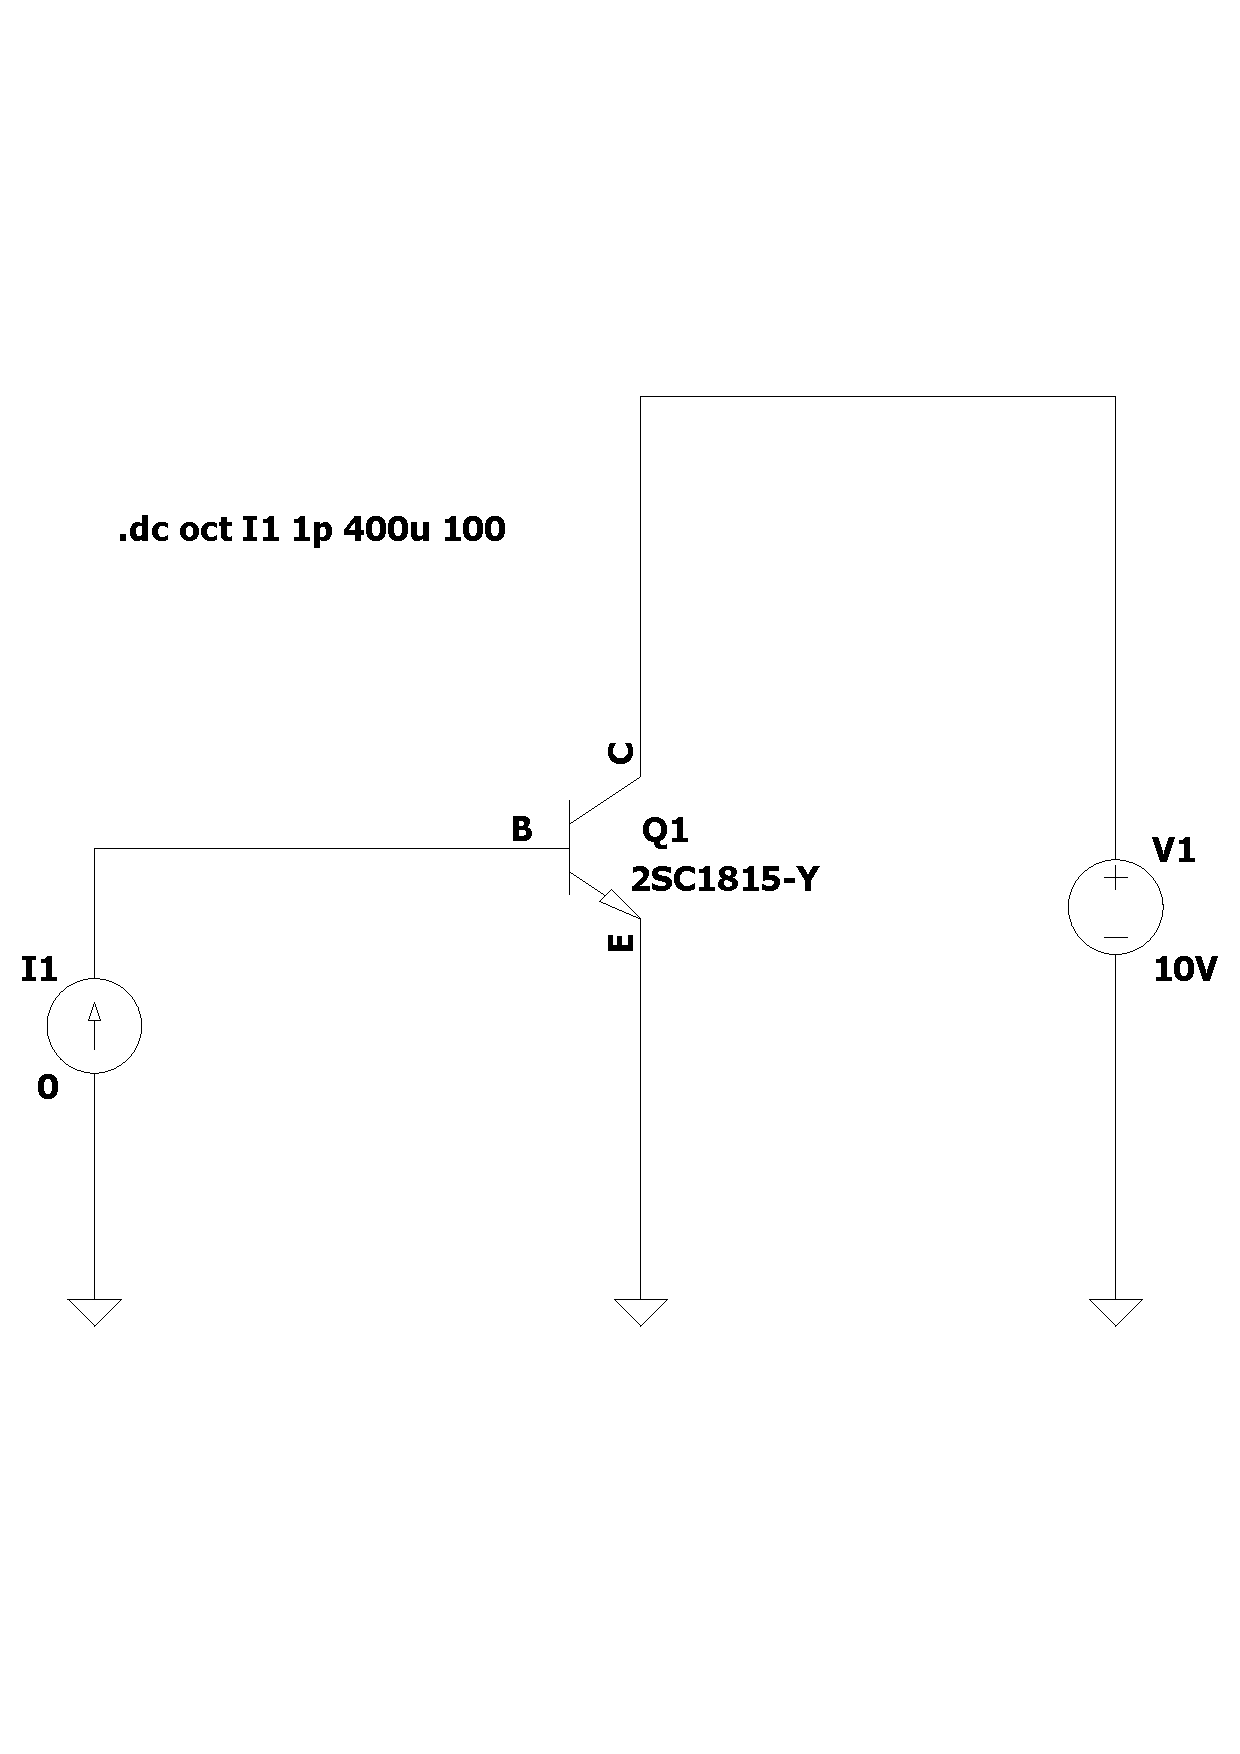
\includegraphics[width=.45\columnwidth]{img/25.pdf}
    }

    \subfigure[dcディレクティブタブ]{
    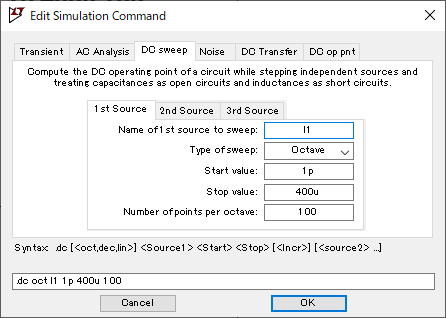
\includegraphics[width=.45\columnwidth]{img/26.png}
    }
    \subfigure[DCスイープ]{
    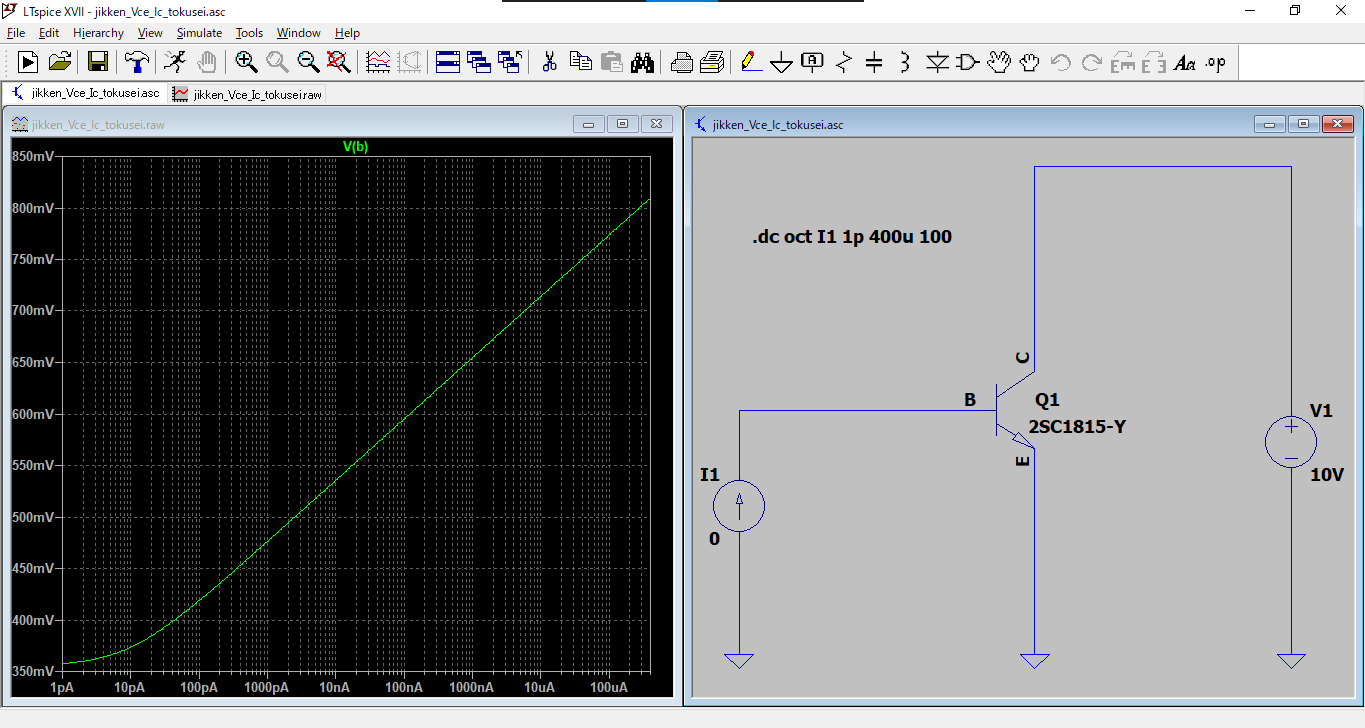
\includegraphics[width=.45\columnwidth]{img/27.png}
    }
    \caption{$I_E$-$V_{BE}$特性の取得方法} 
    \label{tejun1}
    \end{center}
  \end{figure}
  \item 「Run」ボタンをクリックして解析を実行する
  \item ベース電圧を測定する(プローブカーソルを合わせてクリックすると、図\ref{tejun1}(c)のような画面になる。)
\end{enumerate}
\vspace{-1\baselineskip}
\mysubsubsection{$I_E$-$V_{BE}$特性}
$I_E$-$V_{BE}$特性を図\ref{ie_vbe}に示す。
\begin{enumerate}
  \setlength{\parskip}{0cm} % 段落間
  \setlength{\itemsep}{0cm} % 項目間
  \item グラフの横軸にマウスカーソルを当てて定規カーソルで右クリック →「Horizontal Axis」→ 「Quantity Plotted」欄を "V(b)" に変更 → OKボタンクリックで終了。
  \item グラフの凡例のV(b)をクリック →「Expression Editor」→ 「Enter an algebraic expression to plot」を "-Ie(Q1)" に変更する。
  \item OKボタンをクリックして終了すると -Ie(Q1) vs V(b) のグラフが表示される。
  \item グラフの軸上で右クリックし、「Horizontal Axis」「Vertical Axis」「tick」を調整する。
  \begin{figure}[htb]
    \begin{center}
    \subfigure[$I_E$-$V_{BE}$特性(ダイオード特性)]{
    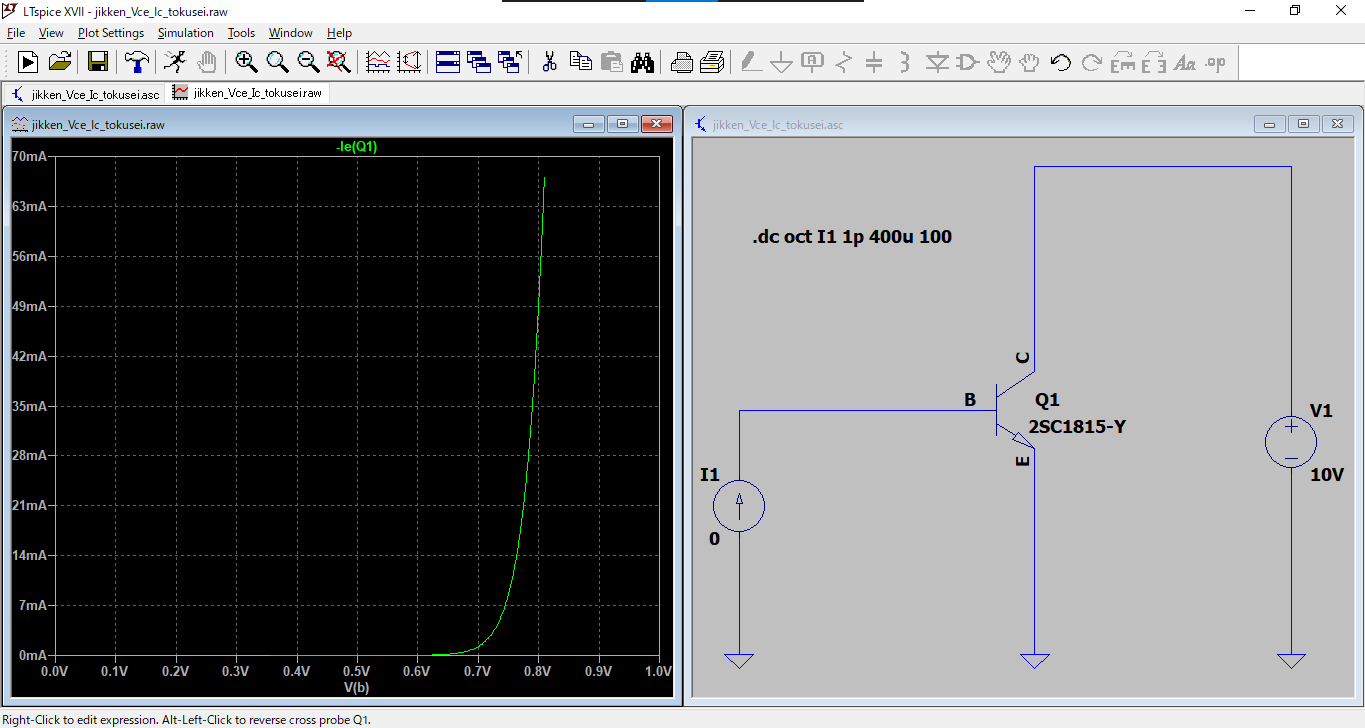
\includegraphics[width=.45\columnwidth]{img/28.png}
    }
    \subfigure[対数表示]{
    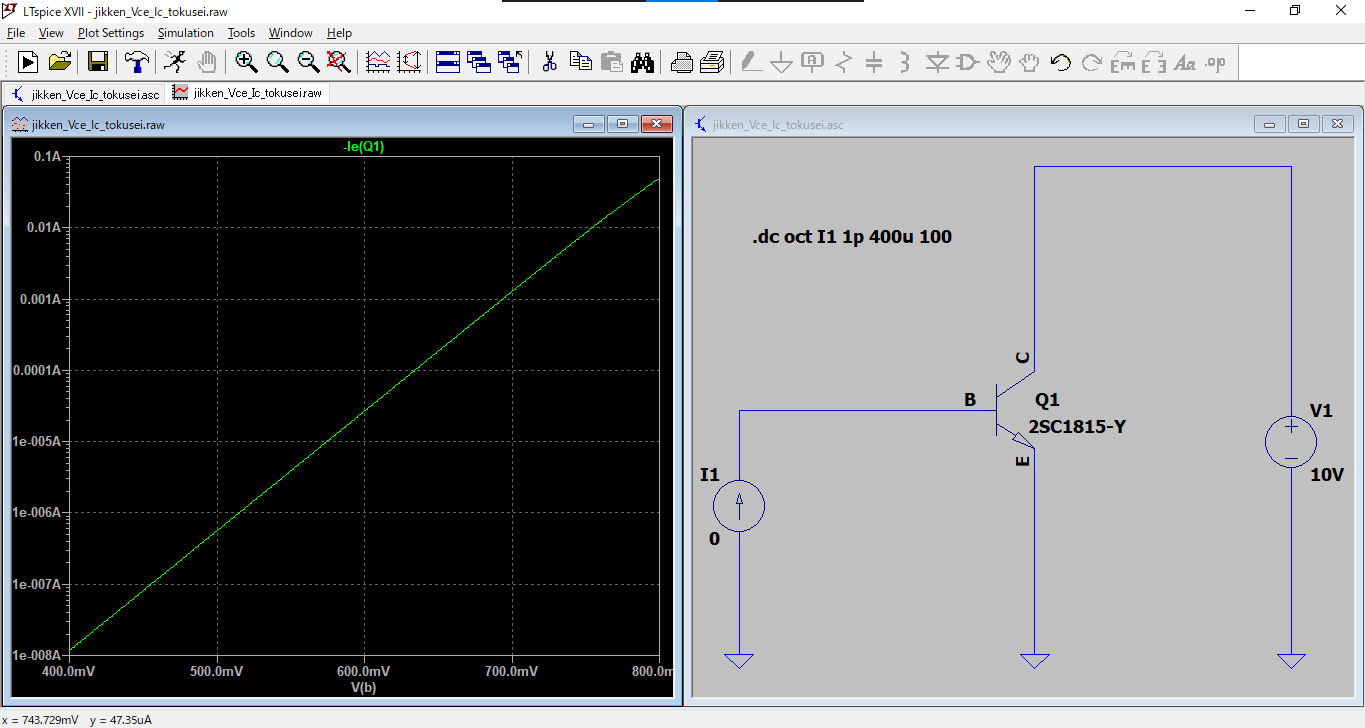
\includegraphics[width=.45\columnwidth]{img/29.png}
    }
    \caption{$I_E$-$V_{BE}$特性}
    \label{ie_vbe}
    \end{center}
  \end{figure}
  \item この特性を印刷するか画像で保存しておく。この回路図も保存しておく。
  \item 「Vertical Axis」→「Logarithmic」欄にチェック → OKと設定すると、片対数グラフでエミッタ電流が直線的に変化している。
\end{enumerate}

\begin{description}
  \setlength{\parskip}{0cm} % 段落間
  \setlength{\itemsep}{0cm} % 項目間
  \item[課題2] 2SC1815の$I_E$-$V_{BE}$特性をDCスイープにより取得して下さい。(用いた回路図とディレクティブを示すこと。図\ref{tejun1}(a)(c)、図\ref{ie_vbe}(a)(b)
  \item[任意課題4] 片対数グラフを用いて、$\frac{q}{kT}\log_{10}(e)$の値(理論値)と比較してください。\\
  カーソルを用いて傾きを求める。グラフ上部の凡例を右クリック →「Expression Editor」→「Attached Cursor」→ 1st \verb|&| 2nd を選んで十字カーソルを2個表示
\end{description}
\vspace{-0.5\baselineskip}
\mysubsubsection{$I_C$-$I_B$特性}
$I_C$-$I_B$特性を図\ref{ic_ib}に示す。「Edit Simulation Cmd」→ 「Edit Simulation Command」→「DC sweep」で以下のように設定しディレクティブを貼り付ける。
  \begin{figure}[htb]
    \begin{center}
    \subfigure[DCスイープ設定]{
    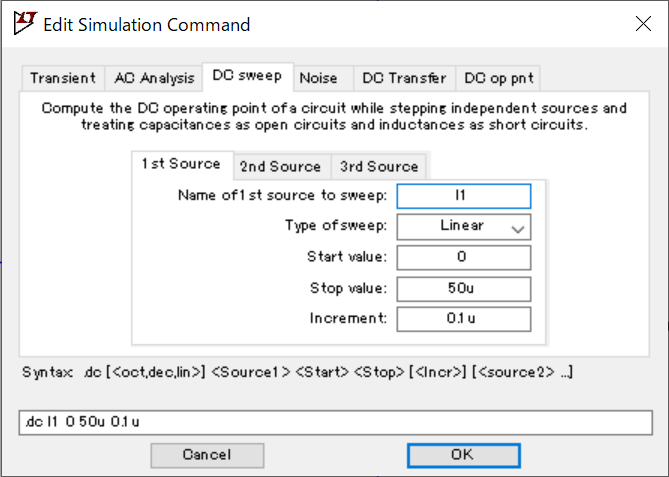
\includegraphics[width=.45\columnwidth]{img/30.png}
    }
    \subfigure[$I_C$-$I_B$特性]{
    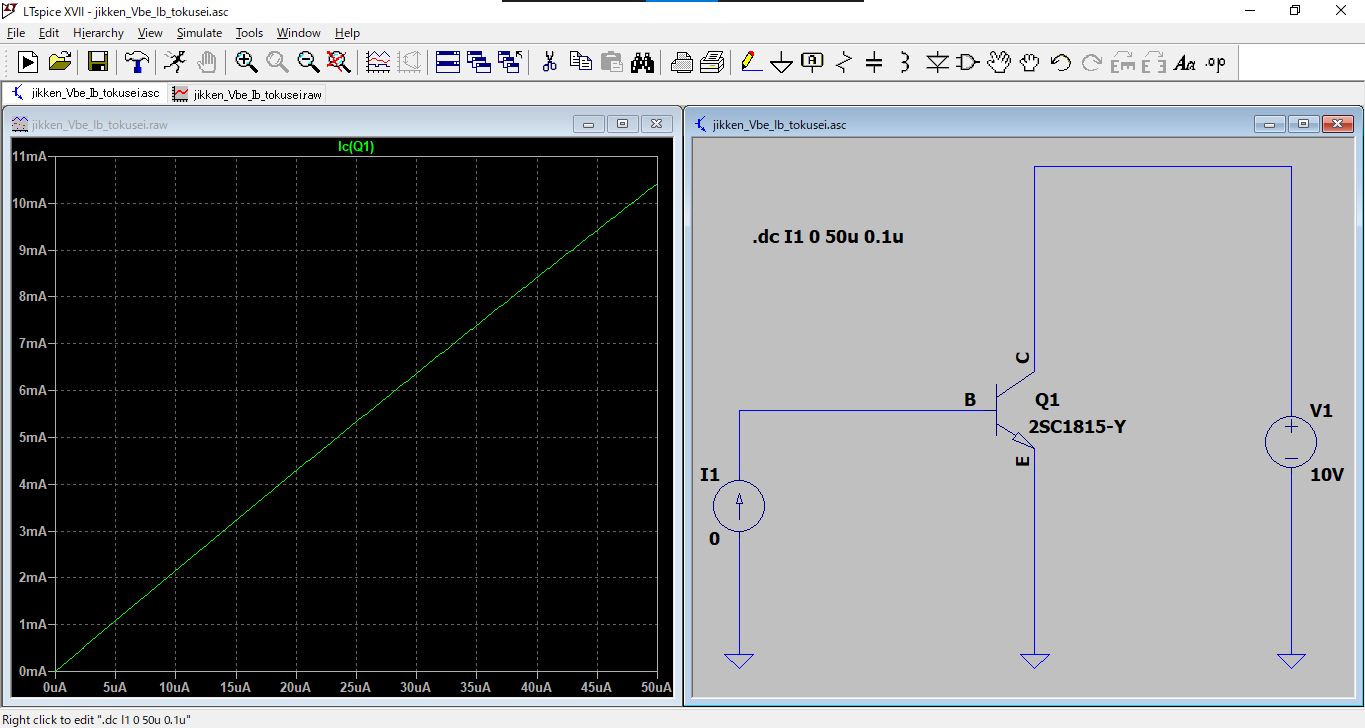
\includegraphics[width=.45\columnwidth]{img/31.png}
    }
    \caption{$I_C$-$I_B$特性}
    \label{ic_ib}
    \end{center}
  \end{figure}

\begin{description}
  \setlength{\parskip}{0cm} % 段落間
  \setlength{\itemsep}{0cm} % 項目間
  \item[課題3] 2SC1815の$I_C$-$I_B$特性をDCスイープにより取得して下さい。(用いた回路図とディレクティブを示すこと。図\ref{ic_ib}(a)(b)
  \item[任意課題5] $I_C-I_B$ 特性を用いてエミッタ交流電流増幅率と接地直流電流増幅率を求めて下さい。その値を直流電流増幅率と比較して下さい。
  \item[交流電流増幅率] 特性曲線の1点で、ベース電流とコレクタ電流の増幅率を求める。
  \item[直流電流増幅率] 特性曲線の2点で、ベース電流とコレクタ電流の増幅率を求める。
\end{description}
\vspace{-1\baselineskip}
\mysubsubsection{$I_C$-$V_{CE}$特性}
$I_C$-$V_{CE}$特性を取得するためのopディレクティブの設定を図\ref{ic_vce_op}、$I_C$-$V_{CE}$特性を図\ref{ic_vce}に示す。
\begin{enumerate}
  \setlength{\parskip}{0cm} % 段落間
  \setlength{\itemsep}{0cm} % 項目間
  \item $I_1$をパラメータとして設定する。$I_1$を右クリックして \verb|"{IB}"| と入力する。
  \item spiceディレクティブを設定
    \begin{itemize}
      \setlength{\parskip}{0cm} % 段落間
      \setlength{\itemsep}{0cm} % 項目間
      \item 「SPICE Directive」(.op) → 「Edit Text on the Schematic」→ 入力欄で右クリック「Help me Edit」→ 「.step Command」→ 「.step Statement Editor」にSPICEディレクティブを書き込む → OK
      \item \verb|.step param IB list 10u 15u 20u 25u 30u 35u 40u 45u 50u| と入力

    \begin{figure}[htb]
      \begin{center}

      \subfigure[$I_C$-$V_{CE}$特性]{	% 副題なし
      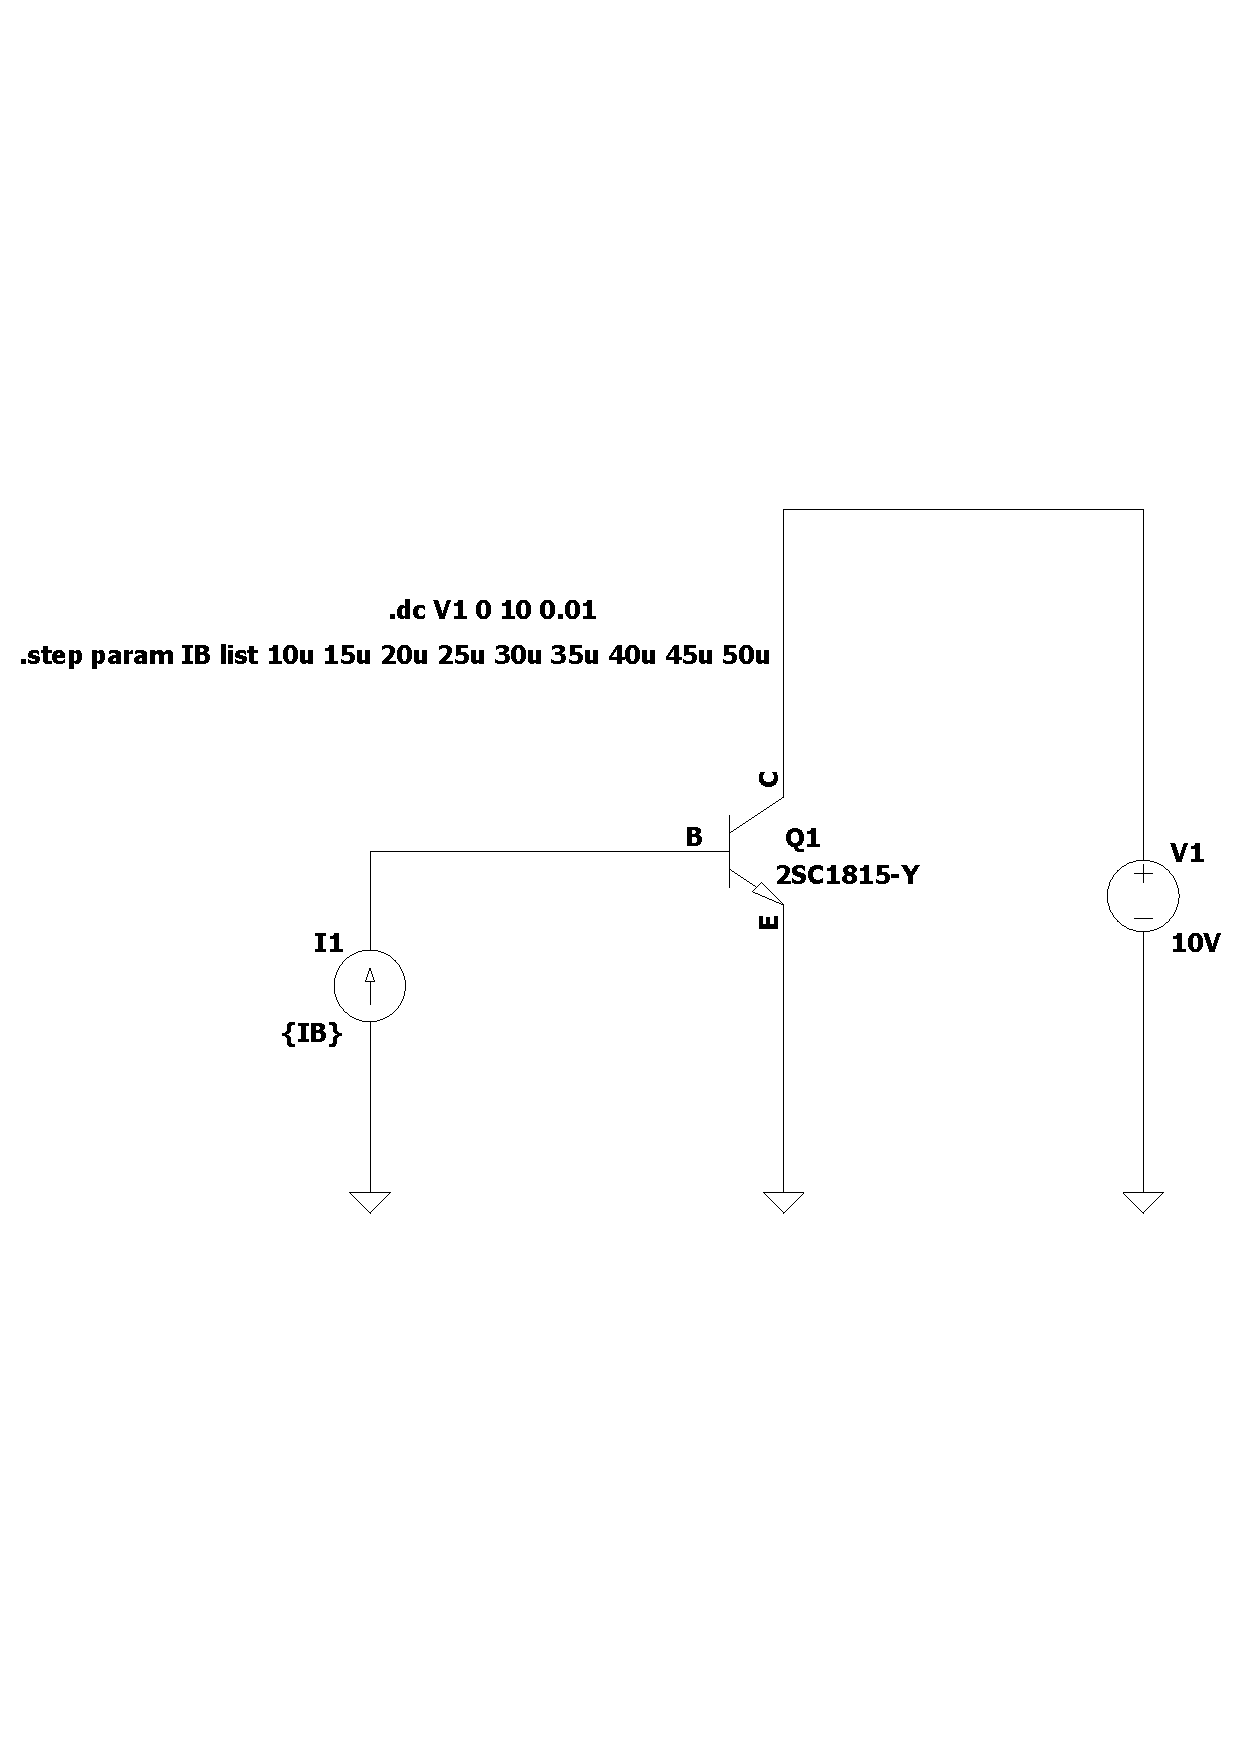
\includegraphics[width=.7\columnwidth]{img/32.pdf}
      }
      \subfigure[.op ディレクティブ]{
      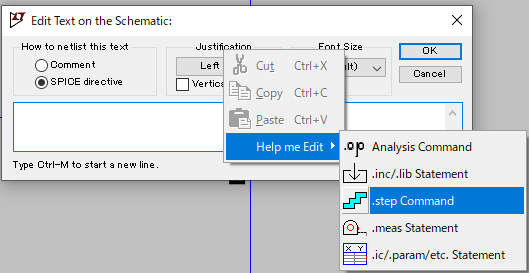
\includegraphics[width=.45\columnwidth]{img/33.png}
      }
      \subfigure[stepパラメータの設定]{
      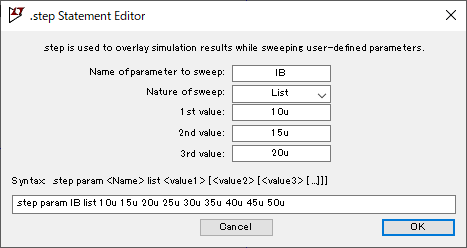
\includegraphics[width=.45\columnwidth]{img/34.png}
      }
      \caption{.op ディレクティブの設定}
      \label{ic_vce_op}
      \end{center}
    \end{figure}
  \end{itemize}
  \item DCスイープの設定
  \begin{itemize}
    \setlength{\parskip}{0cm} % 段落間
    \setlength{\itemsep}{0cm} % 項目間
    \item \verb|.dc V1 0 10 0.01|
    \item 「Run」をクリックし、$I_C$をプローブで測る。
  \end{itemize}
  \begin{figure}[htb]
    \begin{center}
    \subfigure[$I_C$-$V_{CE}$特性の.opディレクティブ実行結果]{
    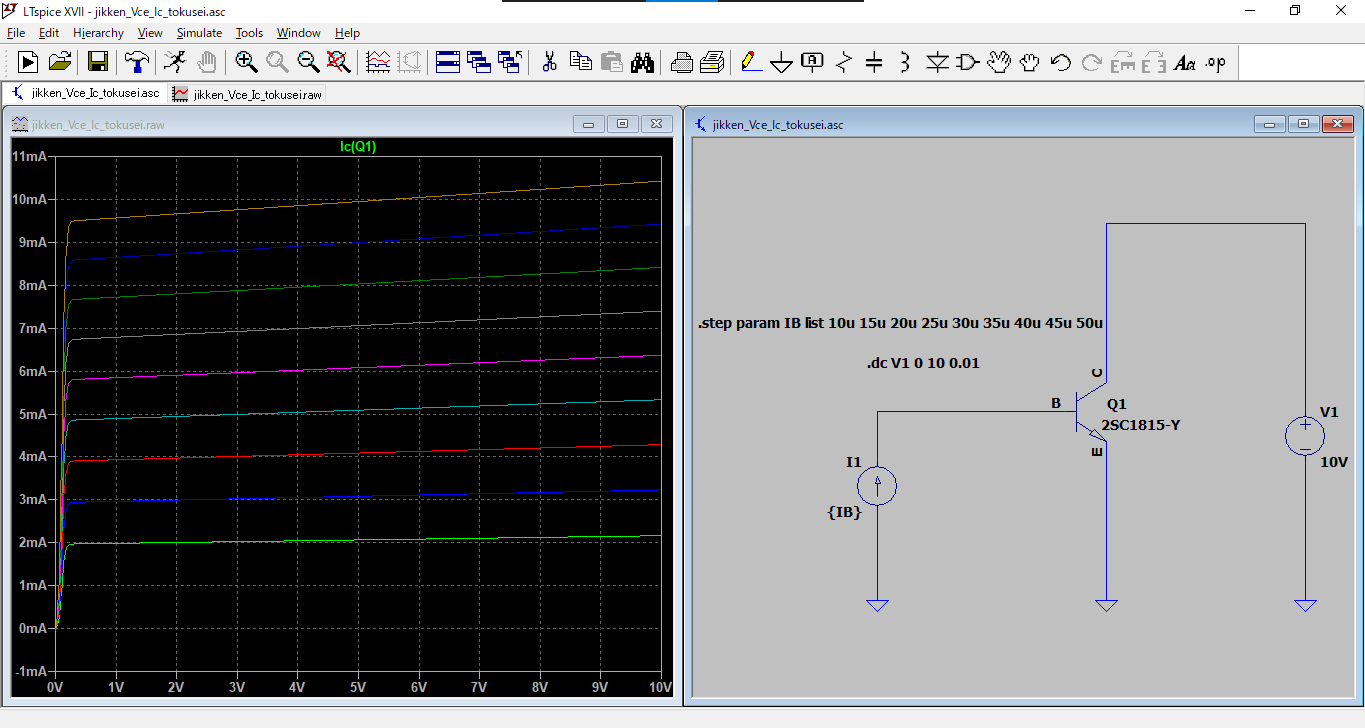
\includegraphics[width=.55\columnwidth]{img/35.png}
    }
    \subfigure[$I_C$-$V_{CE}$特性]{
    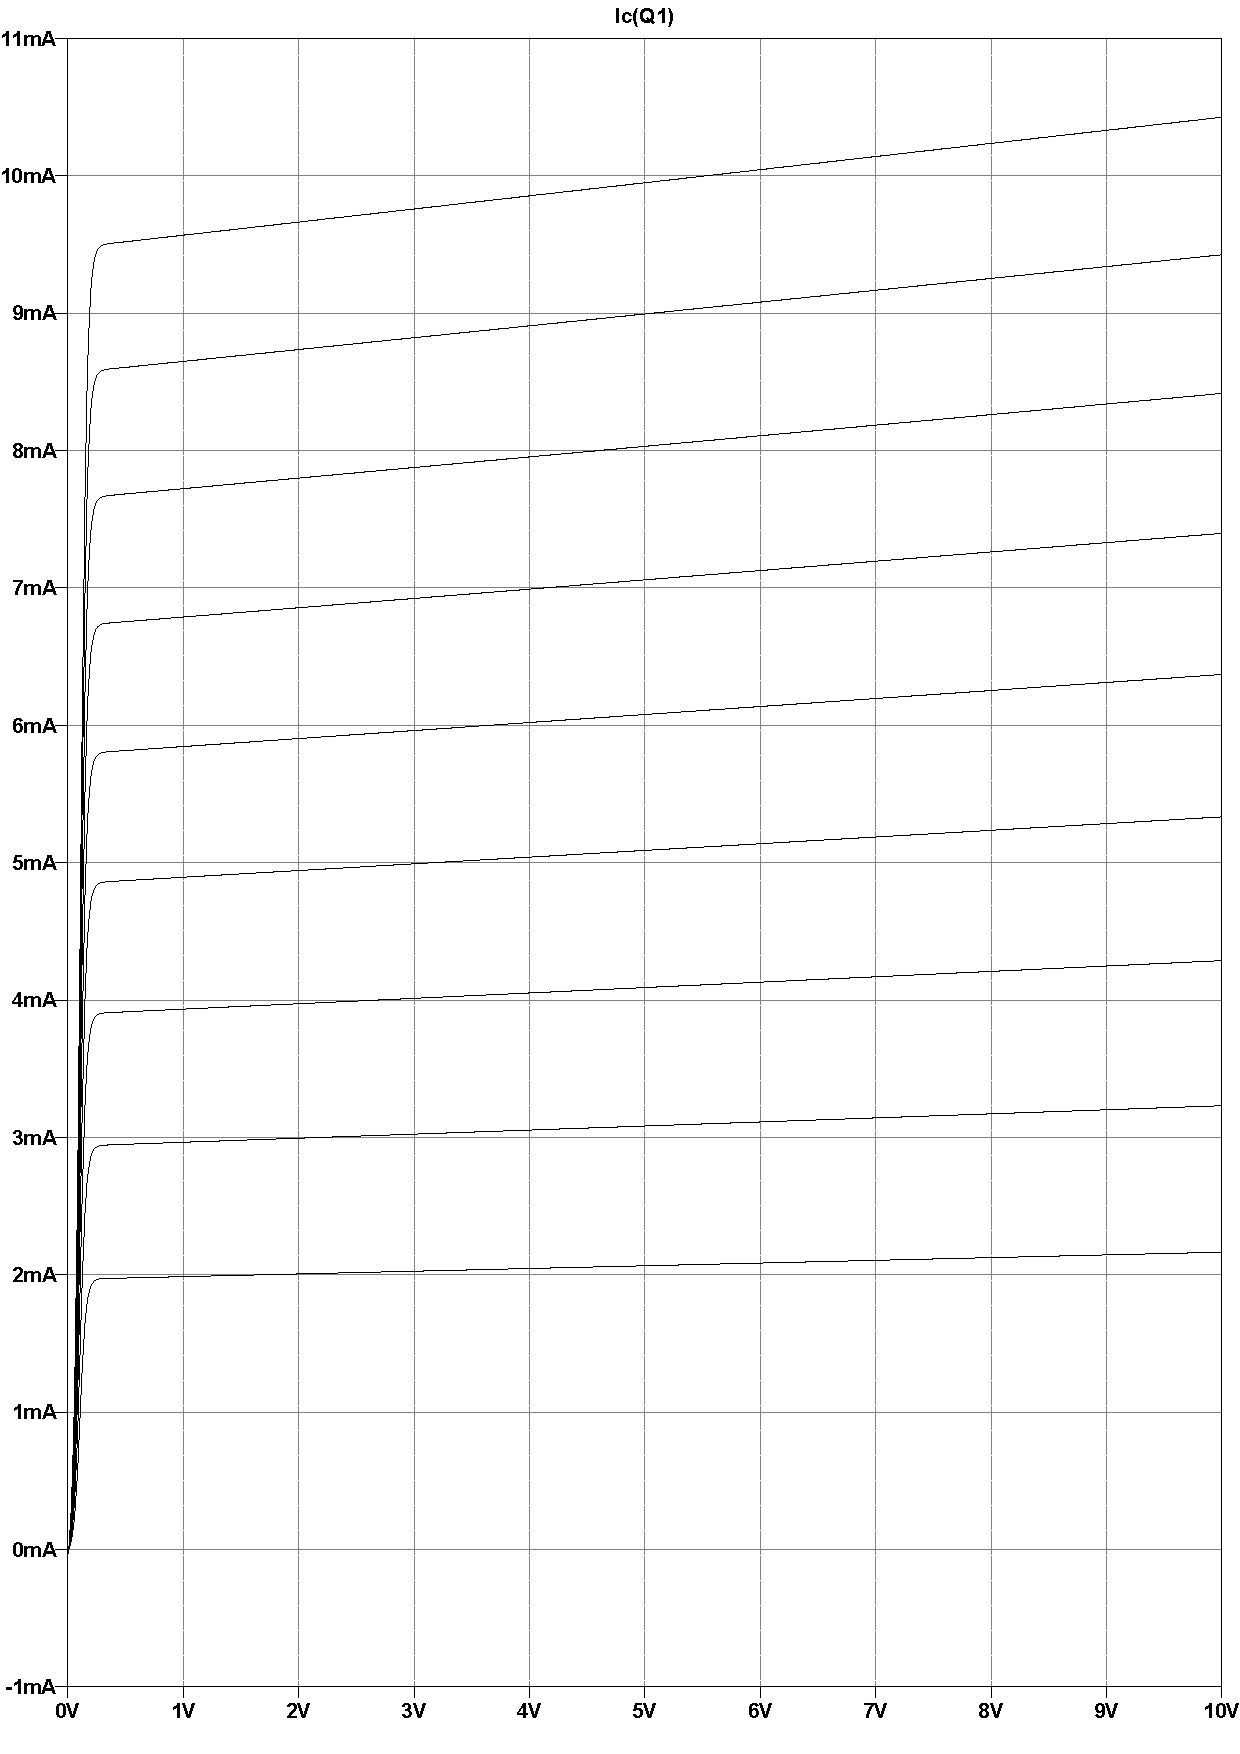
\includegraphics[width=.35\columnwidth]{img/36.pdf}
    }
    \caption{$I_{CE}$-$V_{CE}$特性}
    \label{ic_vce}
    \end{center}
  \end{figure}
    \item この特性を印刷するか画像で保存しておく。
    \begin{description}
      \setlength{\parskip}{0cm} % 段落間
      \setlength{\itemsep}{0cm} % 項目間
      \item[課題4] 2SC1815の$I_C$-$V_{CE}$ 特性をSPICEディレクティブを用いて取得して下さい。(用いた回路図とディレクティブを示すこと。図\ref{ic_vce_op}(a)、図\ref{ic_vce}(a)(b))
      \item[任意課題6] $I_C$-$V_{CE}$ 特性から、入力信号トランジスタの増幅回路を設計するための$V_{CE}$の領域は何 V \verb|~| 何 V が良いでしょうか?
    \end{description}
\end{enumerate}
% \mysection{エミッタ接地回路のバイアス電圧$v_{be}$の設定}
エミッタ接地回路の動作点設定を、原理の説明とシミュレーションによる演習により理解する。

\begin{description}
  \setlength{\parskip}{0cm} % 段落間
  \setlength{\itemsep}{0cm} % 項目間
  \item[ゴール] 2電源バイアス回路をLTSpiceで設計する。(バイアス電圧$V_{be}$と負荷抵抗$R_L$を決定する。)
  \item[キーワード] $I_C$-$V_{CE}$特性、$I_E$-$V_{BE}$ 特性、負荷線、動作点 $V_{CEO}$・$I_{CO}$・$V_{BEO}$
  \item[ストーリー] $I_E$-$V_{BE}$特性と、$I_C$-$V_{CE}$特性を使って、動作点 $V_{CEO}$・$I_{CO}$・$V_{BEO}$ を決める。→ 過渡解析により増幅率を実測 → 計算値と比較。
\end{description}

\mysubsection{演習手順}
原理で計算した値を用いて図\ref{2den_kaiseki}(a)に示す回路図を設計する。入力信号は正弦波$v_{be} = 5.27$ mVp-p を使用する。

\begin{figure}[htb]
  \begin{center}
  \subfigure[2電源バイアス回路の動作点]{	% 副題なし
  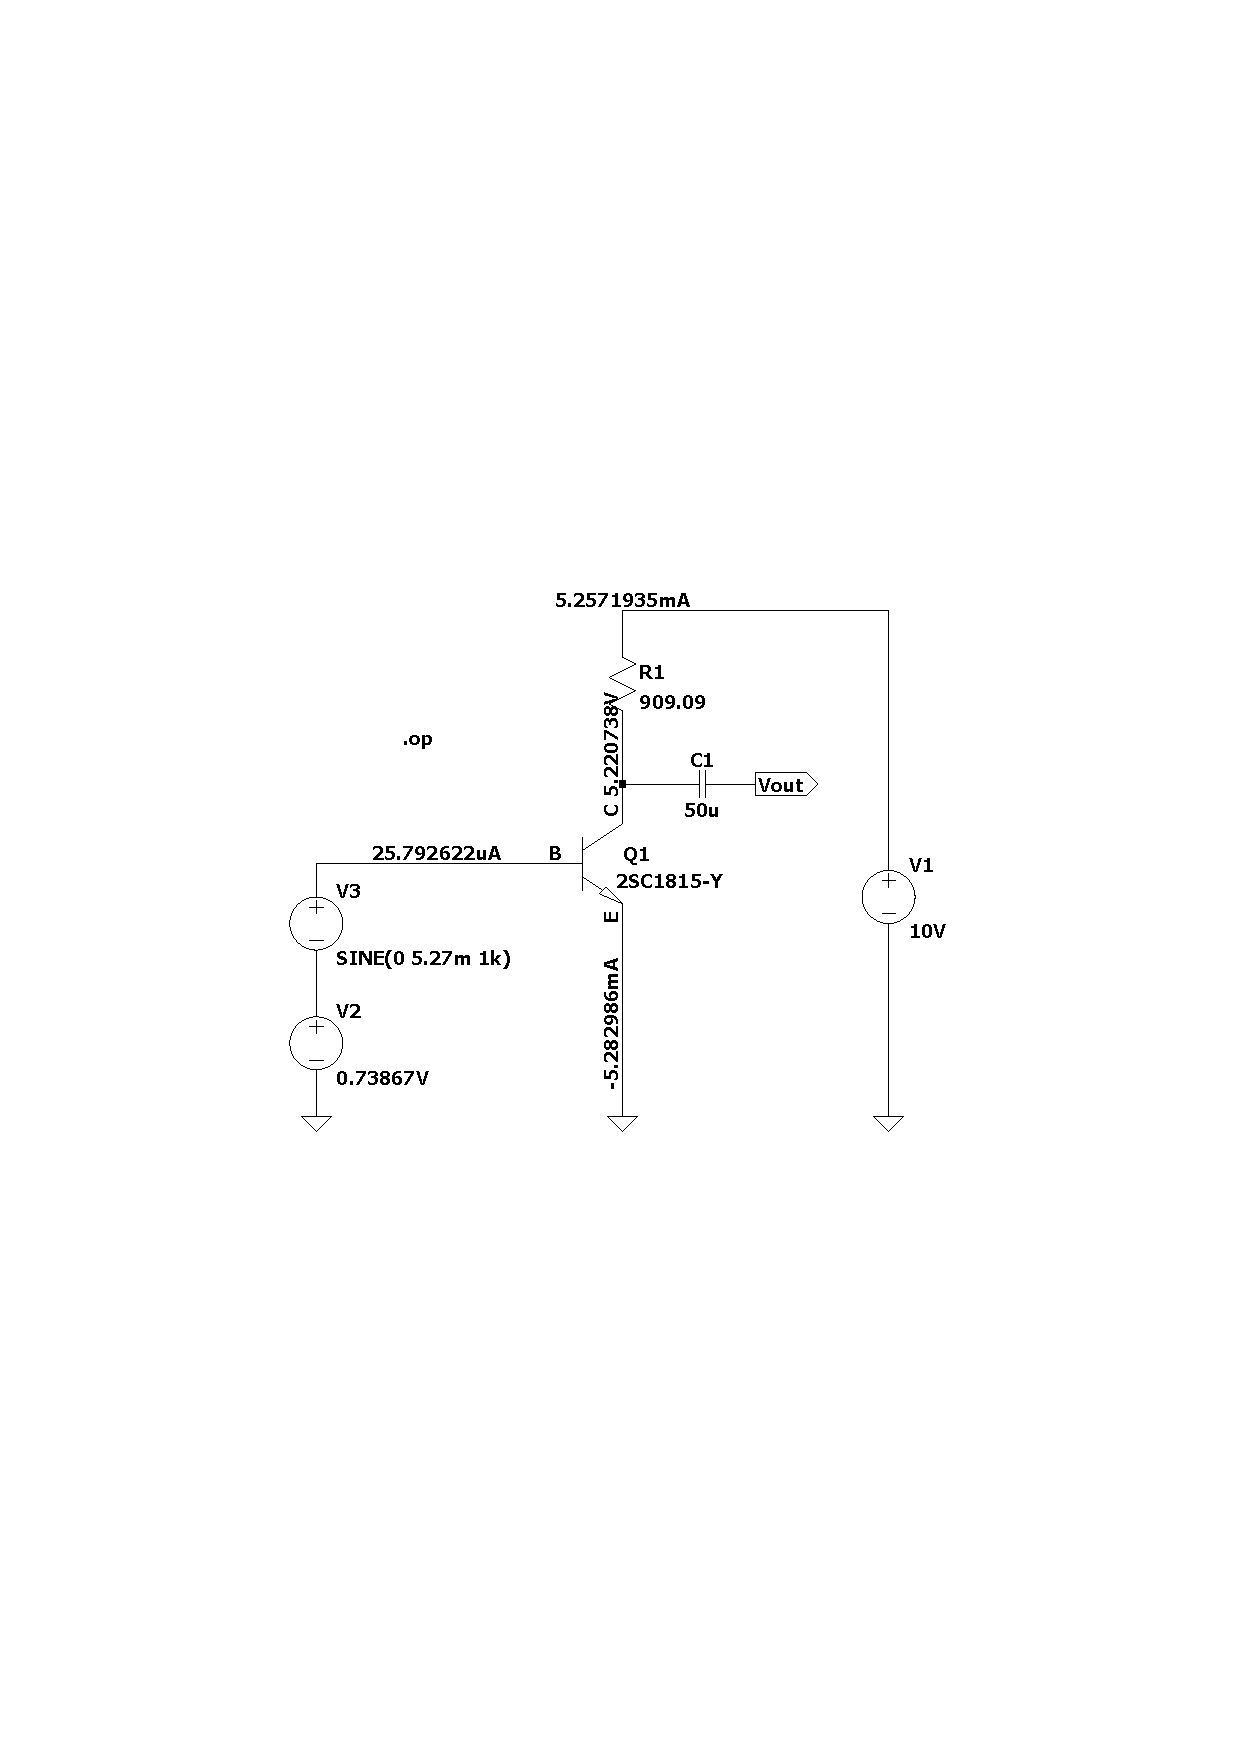
\includegraphics[width=.5\columnwidth]{img/40.pdf}
  }~
  \subfigure[動作点解析結果]{
  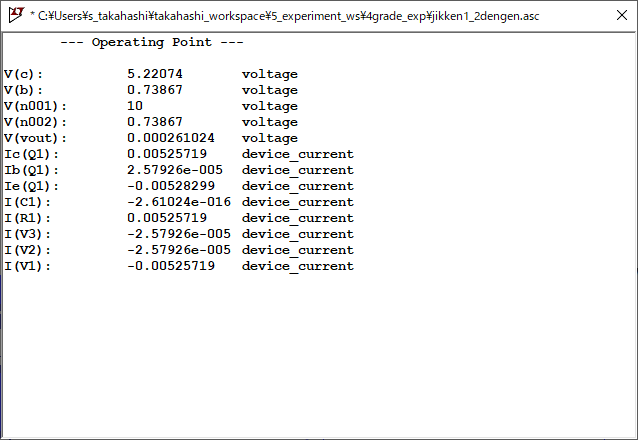
\includegraphics[width=.5\columnwidth]{img/41.png}
  }
  \subfigure[過渡解析結果]{
  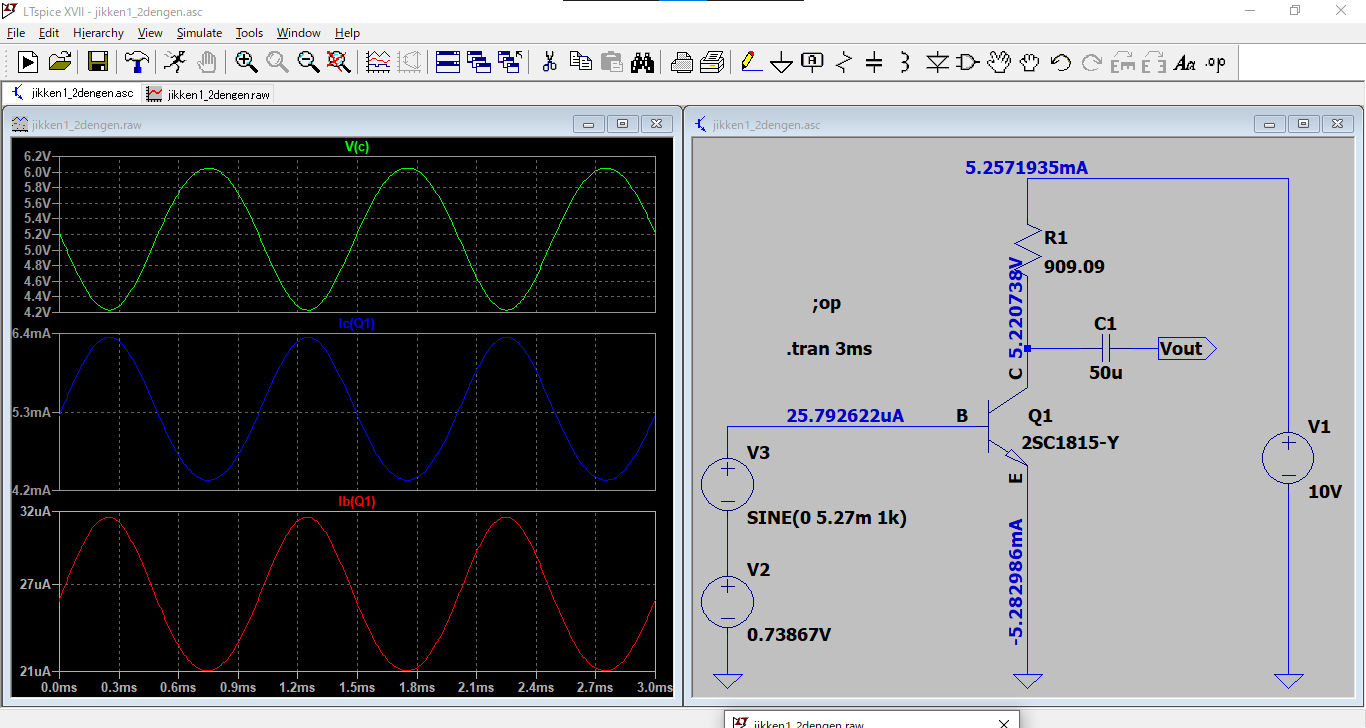
\includegraphics[width=.8\columnwidth]{img/42.png}
  }
  \caption{2電源バイアス回路の各種特性}
  \label{2den_kaiseki}
  \end{center}
\end{figure}

\mysubsubsection{DC動作点解析}
spiceディレクティブ「DC op pnt」に ".op" のみ記述し、ディレクティブに張り付ける → 「Run」で実行。→ 設計した値に対応するベース電流、コレクタ電流がDC動作点の解析結果として現れる。

\begin{description}
  \setlength{\parskip}{0cm} % 段落間
  \setlength{\itemsep}{0cm} % 項目間
  \item[課題5] 2SC1815のDC動作点解析を行ってください。
  (ベース電流、コレクタ電流のDC動作点を求める。)(用いた回路図とディレクティブを示すこと。図\ref{2den_kaiseki}(a)(b))
  動作点が正しく設定されているかどうか根拠と共に説明してください。
  直流電流増幅率$\beta_0$を求めて、計算値と比較して下さい。
\end{description}

\mysubsubsection{過渡解析}
「Edit Simulation cmd.」から Transient 解析を選び、「.tran 3ms」ディレクティブを適用させて、過渡解析を実行する。
この時、$V_C、I_C、I_B$ の波形を確認する。


\begin{description}
  \setlength{\parskip}{0cm} % 段落間
  \setlength{\itemsep}{0cm} % 項目間
  \item [課題6] 2SC1815の過渡解析を行ってください。(用いた回路図とディレクティブを示すこと。図\ref{2den_kaiseki}(c))
  $i_b$、$i_c$の波形に対する、$V_{c}$の波形の位相の特徴を説明して下さい。
  交流電流増幅率 $\beta_0$ を求めて下さい。($\beta_0 = i_c/i_b$)
\end{description}
% \mysection{電流帰還バイアス回路の動作点設定}
電流帰還バイアス回路は、エミッタ接地増幅回路の基本形であり、増幅回路の直流電流動作点を決めるための動作原理図である。(実際にこの形のままで使われることはない。)
固定バイアス、自己バイアス等、入力信号(電圧)にバイアスを加える方法はいくつかあるが、一般的に、トランジスタの持つ特性により動作に悪影響を受ける。(直流電流増幅率の温度変化)
この回路は、温度変化による影響を受けにくい設計となっている。

\begin{description}
  \setlength{\parskip}{0cm} % 段落間
  \setlength{\itemsep}{0cm} % 項目間
  \item[ゴール] 前章で決めた動作点と諸条件から直流電流の動作点を決める。(ブリーダ抵抗の値を決定する。)
  \item[キーワード] ブリーダ抵抗、温度補償
  \item[ストーリー] 前章で決めた動作点+諸条件 → 閉路方程式を立てて回路に流れる直流電流を求める。→ 直流電流の動作点を決める。→ LTspice上で設計 → DCスイープにより動作点を確認 → 計算値と比較
\end{description}

\mysubsection{演習手順}
\subsubsection{DC動作点解析}
\begin{description}
  \setlength{\parskip}{0cm} % 段落間
  \setlength{\itemsep}{0cm} % 項目間
  \item [課題7] 図\ref{current_bias_dc}の回路を作成し、.opディレクティブを用いてDC動作点解析をして下さい。(用いた回路図とディレクティブを示すこと。図 6(a)(b))
  DC動作点が正しく設定されているかどうか考えて下さい。
  \begin{figure}[htbp]
    \begin{center}
    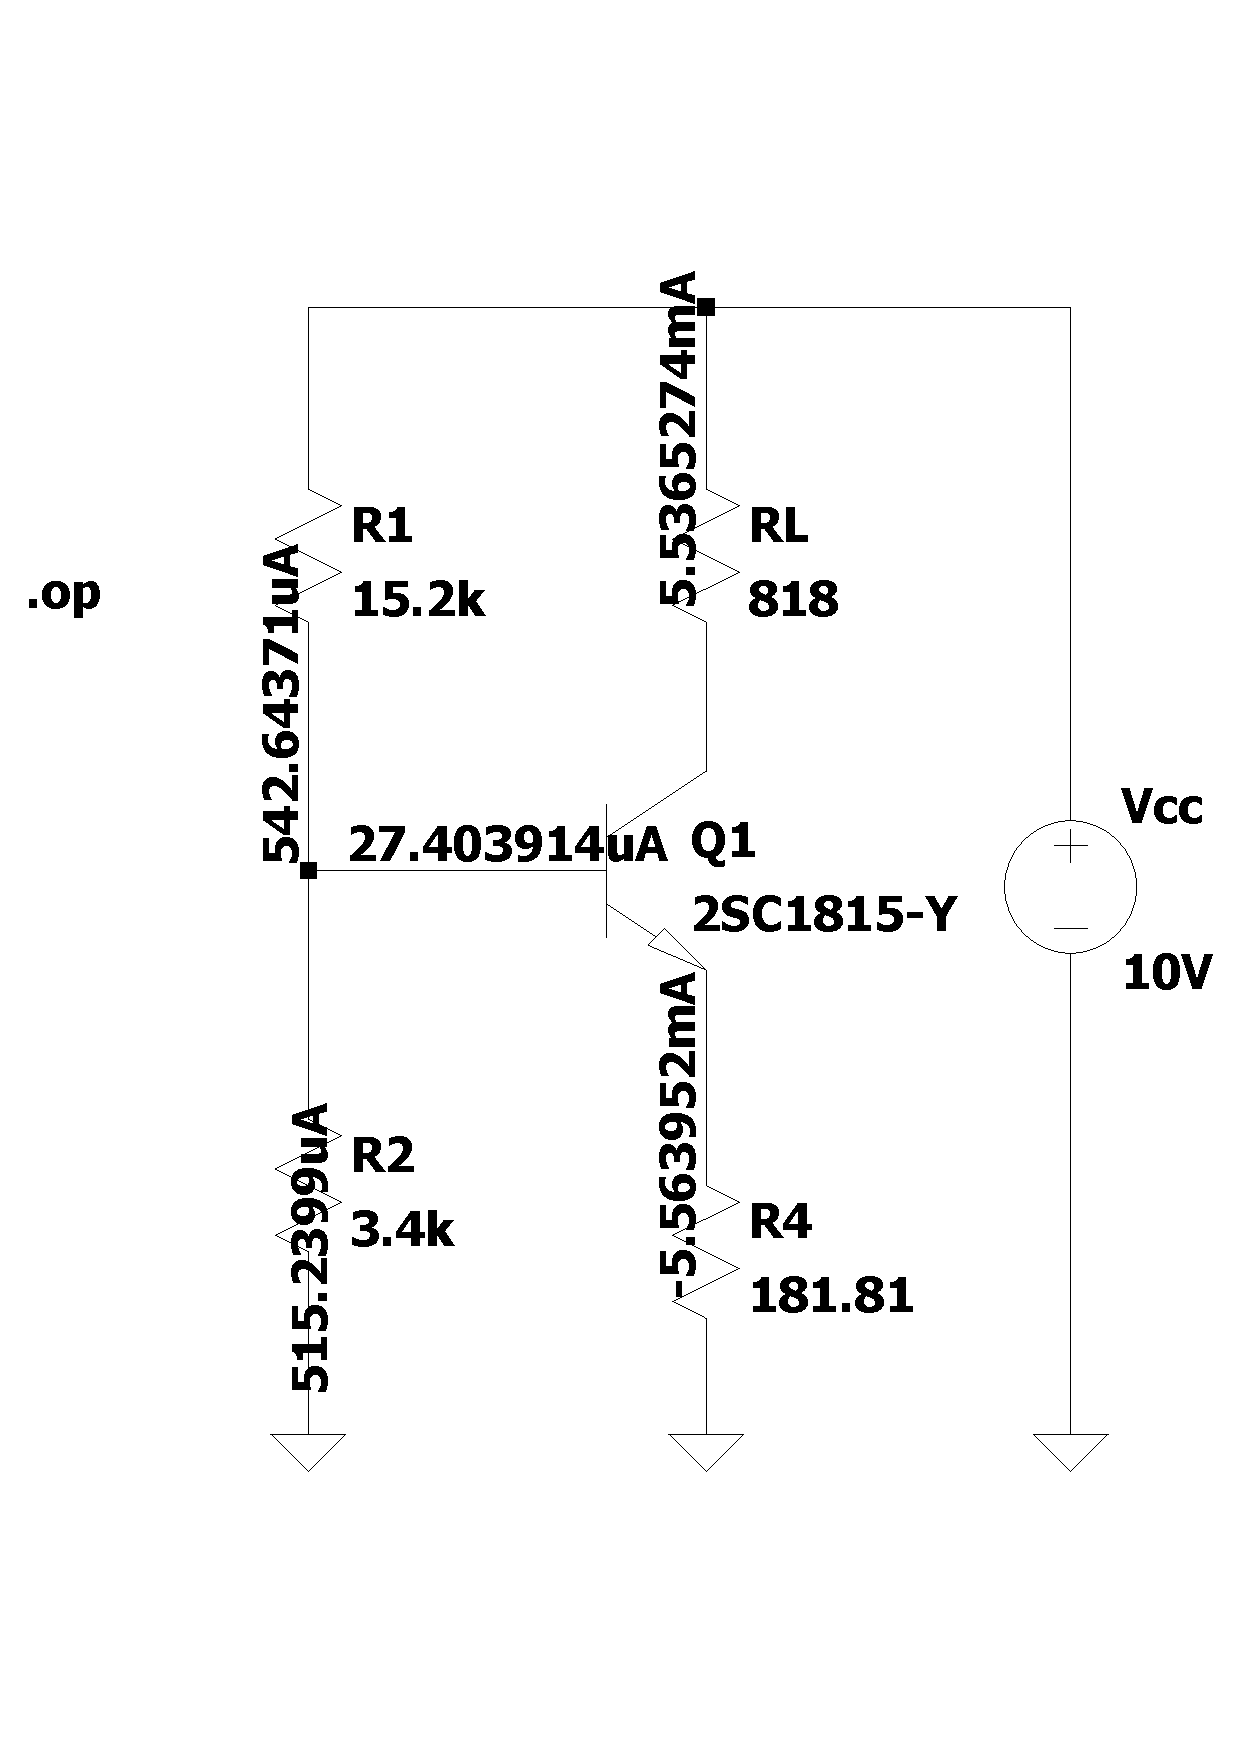
\includegraphics[width=.5\linewidth]{img/44.pdf}
    \caption{電流帰還バイアス回路DC動作点解析}
    \label{current_bias_dc}
    \end{center}
  \end{figure}
\end{description}
% \mysection{エミッタ接地交流増幅回路の設計}
電流帰還バイアス回路を用いたエミッタ接地交流増幅回路を設計する。この回路が、実際に使用されるエミッタ接地回路である。

\begin{description}
  \setlength{\parskip}{0cm} % 段落間
  \setlength{\itemsep}{0cm} % 項目間
  \item[ゴール] 電流帰還バイアス回路を用いたエミッタ接地交流増幅回路を設計する。
  \item[キーワード] 等価回路、結合キャパシタ$C_1、C_2、C_E$、電圧増幅度、遮断周波数、入力インピーダンス、四端子定数、$V_{BE}-I_E$特性
  \item[ストーリー] エミッタ接地回路の交流成分を考える → 交流等価回路にする → 入力インピーダンス、出力インピーダンスをなんか計算する → 低域遮断周波数、電圧増幅度、結合キャパシタの値を決める。ついでに利得とかも計算する。→ LTspiceで設計 → LTspiceで交流増幅特性(AC解析) → LTspiceで過渡解析 → 計算値と比較
\end{description}

\mysubsection{演習手順}
バイアス設定確認 → 動作点解析 → 交流増幅特性解析の順に行う。
$C_2$ の出力側に次段の入力インピーダンス $R_i = 1$k$\Omega$ を接続することで、中域の増幅度が変化する。
\begin{align}
  & 電圧増幅度(中域) |A_v| = \frac{\beta R'_L}{Z_i} = \frac{R'_L}{Z_i/\beta} \approx \frac{R'_L}{r_e}
  (R'_L = R_L//R_i = \frac{R_LR_i}{R_L+R_i}) \\
  & 電圧利得 20 \log (R'_L/r_e)
\end{align}

\mysubsubsection{過渡解析(中域の増幅度に関して)}
\begin{enumerate}
  \setlength{\parskip}{0cm}
  \setlength{\itemsep}{0cm}  
  \item $v_1 = 10$mV (振幅), 1 kHz
  \item $R_i$ の次段の入力抵抗を1k$\Omega$
  \item $R'_L = R_L // R_i$ より、$R_i$ は、中域の増幅度に影響を与える。
\end{enumerate}
中域増幅度 $|A_v| = \frac{\beta R'_L}{Z_i} = \frac{R'_L}{Z_i/\beta} \approx \frac{R'_L}{r_e}$より、
\begin{align}
  R'_L = R_L // R_i = 818.18 // 10^{3} = 449.999... \fallingdotseq 450[\Omega]\\
  電圧増幅率 |A_v| \approx \frac{R'_L}{r_e} = \frac{450}{4.7272...} = 95.1937... \fallingdotseq 95\\
  電圧利得 20\log(\frac{R'_L}{r_e}) = 20\log(\frac{450}{4.7272...}) = 39.572... \fallingdotseq 39.6\textrm{dB}  
\end{align}

\begin{description}
  \item[課題8] 入力信号 $v_1 =$ 20 mVp-p 1kHz として図\ref{kouryu}の回路を設計し、過渡特性を取得して下さい。 \\
  (用いた回路図とディレクティブを示すこと。図\ref{kouryu}(a)(b))
\end{description}

\begin{figure}[htb]
  \begin{center}
  \subfigure[エミッタ接地交流増幅回路]{	% 副題なし
  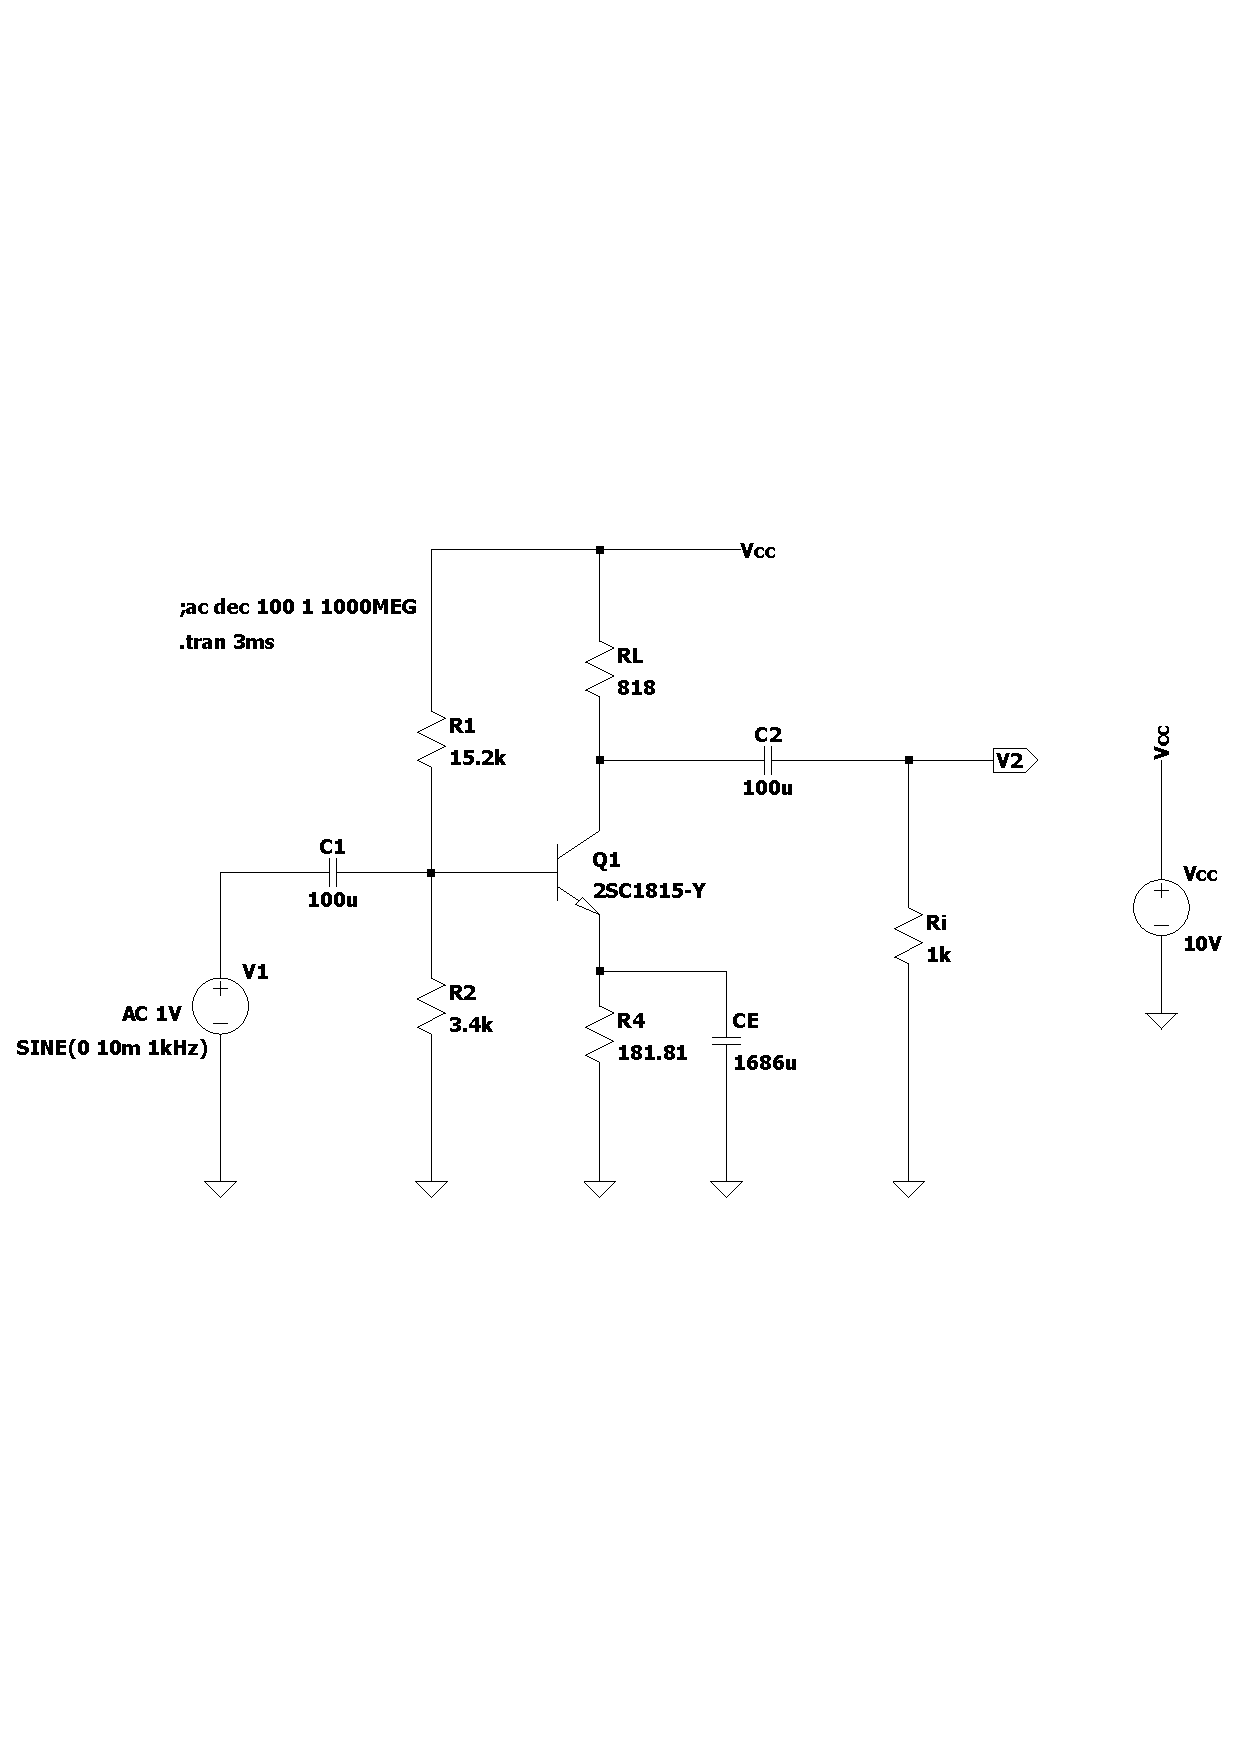
\includegraphics[width=.5\columnwidth]{img/52.pdf}
  }~
  \subfigure[過渡特性結果]{
  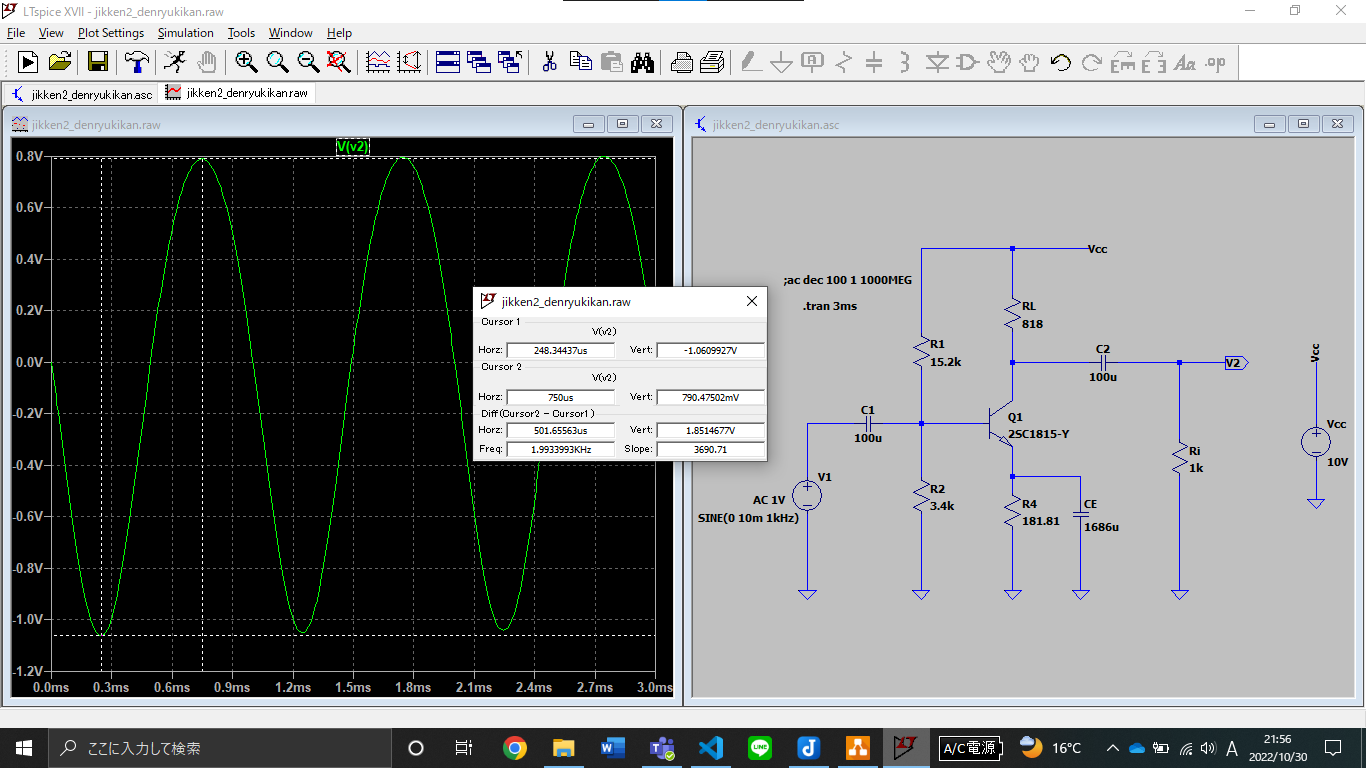
\includegraphics[width=.5\columnwidth]{img/53.png}
  }
  \caption{過渡特性}
  \label{kouryu}
  \end{center}
\end{figure}

\mysubsubsection{AC解析}
\begin{description}
  \item[課題9] 手順に沿って図\ref{ackaiseki}に示すAC解析を行って下さい。\\
「Edit Simulation Command.」→ 「AC解析」→ 「Stop frequency」を"100MEG"に設定 → .ac ディレクティブを回路図に張り付けて「Run」を実行する。
電圧プローブを$v_2$ に設定する。

\begin{figure}[htb]
  \begin{center}
  \subfigure[AC解析結果]{	% 副題なし
  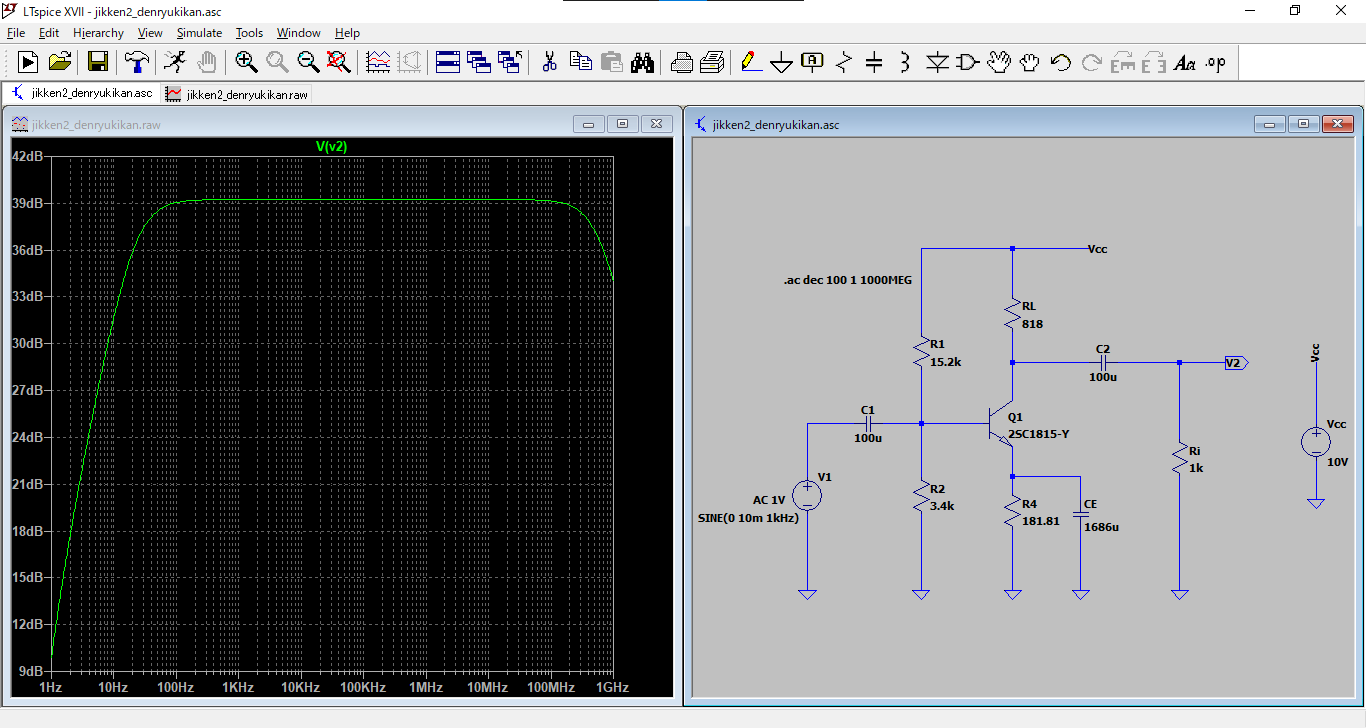
\includegraphics[width=.5\columnwidth]{img/54.png}
  }~
  \subfigure[AC特性(3dB降下をカーソルで取得)]{
  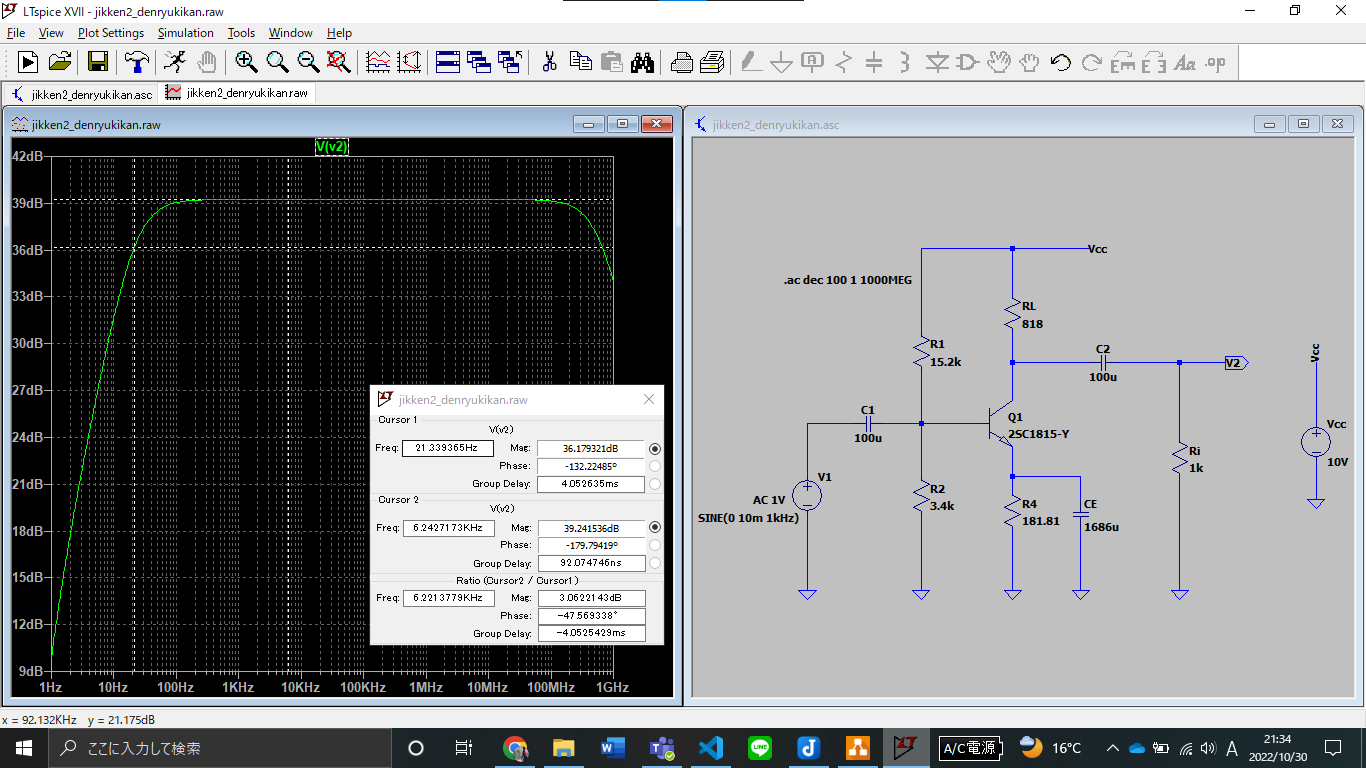
\includegraphics[width=.5\columnwidth]{img/55.png}
  }
  \caption{AC解析}
  \label{ackaiseki}
  \end{center}
\end{figure}

  \item [課題10] 低域遮断周波数、電圧増幅率、電圧利得を計測し、それらの理論値と実測値を比較してください。\\
  低域遮断周波数: 電圧利得が 3dB 降下する周波数\\
  電圧増幅率: 過渡解析において、$v_2$ のp-p 値を求め、$v_2/v_1$ の値を求める。\\
  電圧利得: $20\log|A_v|$ の値をAC解析の中域利得と比較する。

\end{description}

\end{document}